% Created 2024-01-18 Thu 12:21
% Intended LaTeX compiler: pdflatex
\documentclass[presentation]{beamer}
\usepackage[utf8]{inputenc}
\usepackage[T1]{fontenc}
\usepackage{graphicx}
\usepackage{longtable}
\usepackage{wrapfig}
\usepackage{rotating}
\usepackage[normalem]{ulem}
\usepackage{amsmath}
\usepackage{amssymb}
\usepackage{capt-of}
\usepackage{hyperref}
\mode<beamer>{\usetheme{Madrid}}
\definecolor{SUred}{rgb}{0.59375, 0, 0.17969} % SU red (primary)
\definecolor{SUblue}{rgb}{0, 0.17578, 0.38281} % SU blue (secondary)
\setbeamercolor{palette primary}{bg=SUred,fg=white}
\setbeamercolor{palette secondary}{bg=SUblue,fg=white}
\setbeamercolor{palette tertiary}{bg=SUblue,fg=white}
\setbeamercolor{palette quaternary}{bg=SUblue,fg=white}
\setbeamercolor{structure}{fg=SUblue} % itemize, enumerate, etc
\setbeamercolor{section in toc}{fg=SUblue} % TOC sections
% Override palette coloring with secondary
\setbeamercolor{subsection in head/foot}{bg=SUblue,fg=white}
\setbeamercolor{date in head/foot}{bg=SUblue,fg=white}
\institute[SU]{Shenandoah University}
\titlegraphic{\includegraphics[width=0.5\textwidth]{\string~/Documents/suLogo/suLogo.pdf}}
\newcommand{\R}{\mathbb{R}}
\usepackage{tikz}
\usetheme{default}
\author{Chase Mathison\thanks{cmathiso@su.edu}}
\date{22 January 2024}
\title{Precalculus!}
\hypersetup{
 pdfauthor={Chase Mathison},
 pdftitle={Precalculus!},
 pdfkeywords={},
 pdfsubject={},
 pdfcreator={Emacs 29.1 (Org mode 9.6.7)}, 
 pdflang={English}}
\begin{document}

\maketitle

\section{Announcements}
\label{sec:org8e08b18}
\begin{frame}[label={sec:org4e2dcae}]{Announcements}
\begin{enumerate}
\item Welcome to Precalculus!
\item My office hours this semester: M - F, 10am - 11am in Howe 113
\item Let's do some introductions!
\end{enumerate}
\end{frame}

\section{Lecture}
\label{sec:org254aad7}
\begin{frame}[label={sec:orgef44df6}]{Canvas}
Let's go explore in Canvas for a few minutes before we dive into some
material.
\end{frame}

\begin{frame}[label={sec:org7f28464}]{What is an angle?}
\end{frame}

\begin{frame}[label={sec:org72e2a07}]{Drawing an angle}
\begin{definition}[Terminology]
\begin{itemize}
\item Ray
\item Angle
\item Vertex
\item Initial side
\item Terminal Side
\end{itemize}
\end{definition}

\vspace{10in}
\end{frame}

\begin{frame}[label={sec:orge3cbc6a}]{The Measure of an Angle}
\begin{definition}[Terminology]
\begin{itemize}
\item Measure of an angle
\item Degree
\end{itemize}
\end{definition}
\vspace{10in}
\end{frame}

\begin{frame}[label={sec:orgfba14fa}]{Standard Position}
\begin{definition}[Standard Position for an Angle]
An angle is in ``Standard Position'' if the initial side lines up with the positive \uline{\hspace*{1in}},
and the vertex is at the \uline{\hspace*{1in}} in the \(xy\) plane.
\end{definition}

\vspace{10in}
\end{frame}
\begin{frame}[label={sec:org3792949}]{Example}
Sketch the following angles in standard position:
\begin{enumerate}
\item \(45^{\circ}\)
\item \(120^{\circ}\)
\item \(-135^{\circ}\)
\end{enumerate}

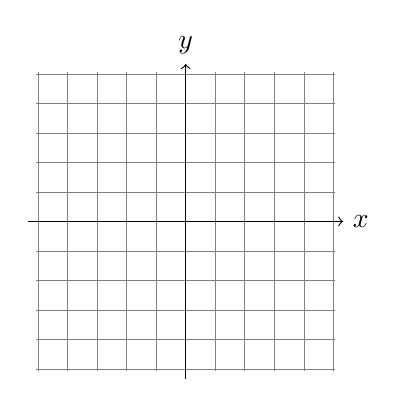
\begin{tikzpicture}
  \draw[step=0.375,help lines](-1.9,-1.9) grid (1.9,1.9);
  \draw[->] (-2,0) -- (2,0) node[anchor=west] {$x$};
  \draw[->] (0,-2) -- (0,2) node[anchor=south] {$y$};
\end{tikzpicture}

\vspace{10in}
\end{frame}

\begin{frame}[label={sec:orgae34f62}]{Radians!}
Degrees are what you're most familiar with to measure an angle, but
the choice of having 360\(^{\circ}\) in a full circular rotation is \uline{\hspace*{1in}}.

A more natural way to measure an angle is to use \uline{\hspace*{1in}}.

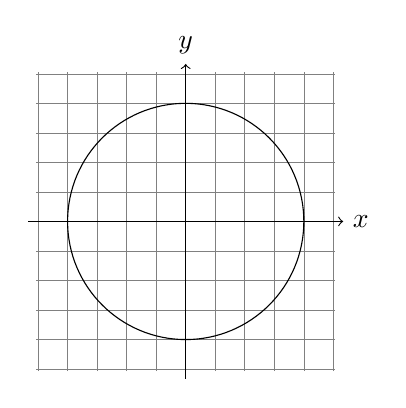
\begin{tikzpicture}
  \draw[step=0.375,help lines](-1.9,-1.9) grid (1.9,1.9);
  \draw[->] (-2,0) -- (2,0) node[anchor=west] {$x$};
  \draw[->] (0,-2) -- (0,2) node[anchor=south] {$y$};
  \draw (0,0) circle [radius=1.5];
\end{tikzpicture}

\vspace{10in}
\end{frame}

\begin{frame}[label={sec:org6551c26}]{Converting Between Radians and Degrees}
\begin{theorem}[Conversion between Radians and Degrees]
\phantom{hi}
\[\]
\phantom{hi}
\end{theorem}

\vspace{10in}
\end{frame}

\begin{frame}[label={sec:org9b3dd4f}]{Example}
Convert:
\begin{enumerate}
\item \(25^{\circ}\) to radians
\item \(\frac{\pi}{3}\) radians to degrees.
\end{enumerate}

\vspace{10in}
\end{frame}

\begin{frame}[label={sec:orgb9264c4}]{Arc Length and Radius}
As we saw above, an angle of \(\theta\) radians corresponds to a
fractional turn of \(\theta = \frac{s}{r}\) around a circle.

We can rearrange this then to say that \(s =\) \uline{\hspace*{1in}}.

\begin{theorem}[Arc length and radius]
If \(\theta\) is an angle measured in radians, then the arc length
\(s\) along a circle of radius \(r\) corresponding to an angle of
\(\theta\) is
\[s = \hspace{1in}\]
\end{theorem}
\end{frame}

\begin{frame}[label={sec:org40f9dde}]{Using Radians}
The circumference of the earth at the equator is 24,901 miles.  Using
this, what is the radius of the earth?

\vspace{10in}
\end{frame}

\begin{frame}[label={sec:org6fc332a}]{Special Angles in Radians}
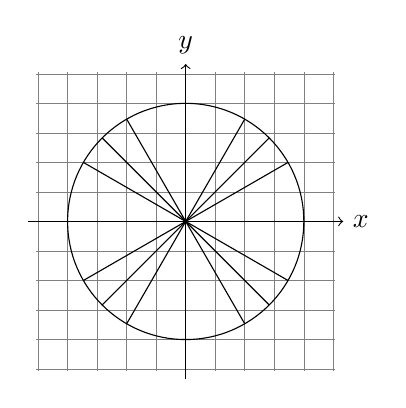
\begin{tikzpicture}
  \draw[step=0.375,help lines](-1.9,-1.9) grid (1.9,1.9);
  \draw[->] (-2,0) -- (2,0) node[anchor=west] {$x$};
  \draw[->] (0,-2) -- (0,2) node[anchor=south] {$y$};
  \draw (0,0) circle [radius=1.5];
  \draw (-1.3,-0.75) -- (1.3,0.75);
  \draw (-1.3,0.75) -- (1.3,-0.75);
  \draw (-1.06,-1.06) -- (1.06,1.06);
  \draw (-1.06,1.06) -- (1.06,-1.06);
  \draw (-0.75,-1.3) -- (0.75,1.3);
  \draw (-0.75,1.3) -- (0.75,-1.3);
\end{tikzpicture}
\end{frame}

\begin{frame}[label={sec:orgb7560d5}]{Coterminal Angles}
\begin{definition}[Coterminal Angles]
\begin{itemize}
\item Coterminal angles
\end{itemize}
\end{definition}

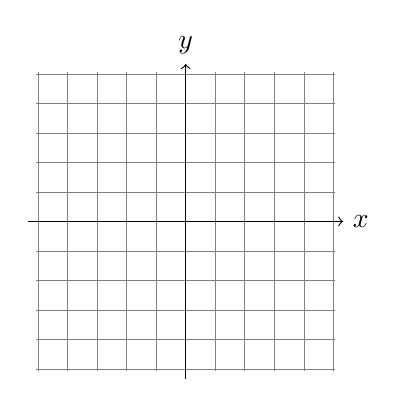
\begin{tikzpicture}
  \draw[step=0.375,help lines](-1.9,-1.9) grid (1.9,1.9);
  \draw[->] (-2,0) -- (2,0) node[anchor=west] {$x$};
  \draw[->] (0,-2) -- (0,2) node[anchor=south] {$y$};
\end{tikzpicture}

\vspace{10in}
\end{frame}

\begin{frame}[label={sec:orga1cf1c5}]{Reference Angles}
\begin{definition}[Reference Angle]
\begin{itemize}
\item Reference Angle
\end{itemize}
\end{definition}

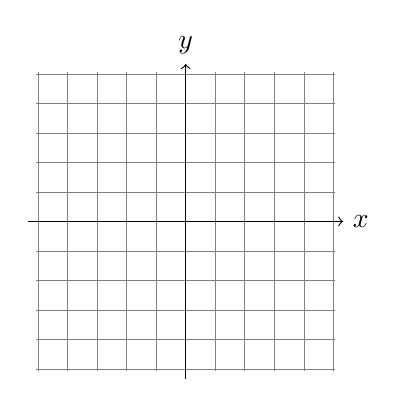
\begin{tikzpicture}
  \draw[step=0.375,help lines](-1.9,-1.9) grid (1.9,1.9);
  \draw[->] (-2,0) -- (2,0) node[anchor=west] {$x$};
  \draw[->] (0,-2) -- (0,2) node[anchor=south] {$y$};
\end{tikzpicture}

\vspace{10in}

\vspace{10in}
\end{frame}

\begin{frame}[label={sec:org7d2d875}]{Examples}
\begin{itemize}
\item Find an angle between 0\(^{\circ}\) and \(360^{\circ}\) that is
coterminal with the angle \(775^{\circ}\).
\item Find the reference angle associated with the angle \(210^{\circ}\).
\end{itemize}

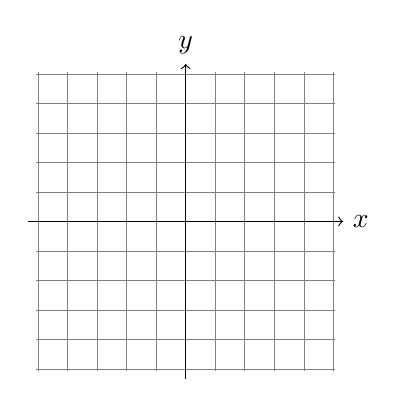
\begin{tikzpicture}
  \draw[step=0.375,help lines](-1.9,-1.9) grid (1.9,1.9);
  \draw[->] (-2,0) -- (2,0) node[anchor=west] {$x$};
  \draw[->] (0,-2) -- (0,2) node[anchor=south] {$y$};
\end{tikzpicture}
\vspace{10in}
\end{frame}

\begin{frame}[label={sec:org69a3c59}]{Coterminal Angles and Reference Angles in Radians}
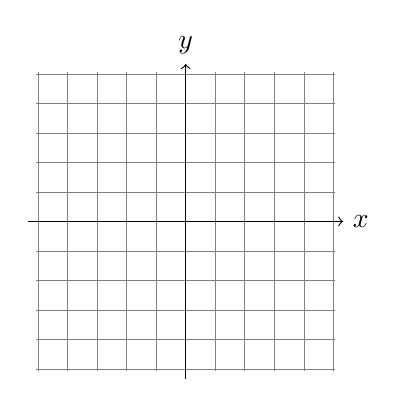
\begin{tikzpicture}
  \draw[step=0.375,help lines](-1.9,-1.9) grid (1.9,1.9);
  \draw[->] (-2,0) -- (2,0) node[anchor=west] {$x$};
  \draw[->] (0,-2) -- (0,2) node[anchor=south] {$y$};
\end{tikzpicture}
\vspace{10in}
\end{frame}

\begin{frame}[label={sec:org3ee0d3c}]{Examples}
\begin{itemize}
\item Find an angle between 0 radians and \(2\pi\) radians that is
coterminal with the angle \(\frac{17\pi}{6}\) radians.
\item Find the reference angle associated with the angle \(\frac{15\pi}{18}\).
\end{itemize}

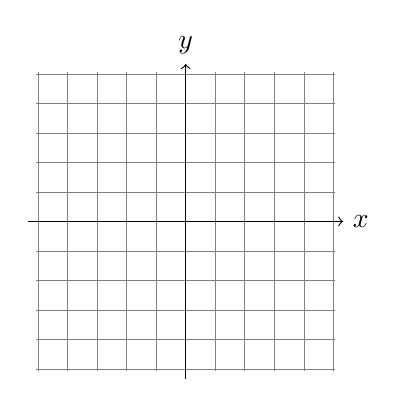
\begin{tikzpicture}
  \draw[step=0.375,help lines](-1.9,-1.9) grid (1.9,1.9);
  \draw[->] (-2,0) -- (2,0) node[anchor=west] {$x$};
  \draw[->] (0,-2) -- (0,2) node[anchor=south] {$y$};
\end{tikzpicture}
\vspace{10in}
\end{frame}
\end{document}